Differentiating quark-initiated (quark) jets from gluon-initiated (gluon) jets is import for VBF \Hbb search as the signal final state includes two VBF quark jets while a big portion of the QCD backgrounds contain final state gluons as discussed in Chapter\ref{chap:vbf}. The key difference between quark and gluon jets is that the Altarelli-Parisi splitting functions~\cite{Altarelli:1977zs} contain a factor of $C_A=3$ for gluon radiation from a gluon and a factor of $C_F=4/3$ for gluon radiation from a quark. Due to this difference, gluon jets tend to have more constituents and a broader radiation pattern than quark jets. A simple sensitivity study in Fig.\ref{fig:cnn-gain} shows that for the \twocentral channel of the VBF \Hbb search\ref{sec:vbf-evtsel}, a reasonalbe quark gluon tagging tool with 15 gluon rejection at 70\% quark efficiency applied to the forward jet can help improve the analysi sensitivity ($s/\sqrt{b}$) by $7\%$ (more gain expected if applied to both VBF jets and to \fourcentral).

Most of the prior experimental studies have focused on devising a small number of key jet level observables that capture this difference. Variables such as \ntrk, whic is the number of tracks within a jet, has been used in VBF \Hbb search \ref{sec:vbf-bdt} and improved the overall sensitivity for the analysis. However, such high level representation of jet information may not capture the spatial and internal structure of jets. Prior works such as ~\cite{deOliveira:2015xxd} has suggested that an image representation of the jets with high granularity such that most of the individual costituent are visible could provide richer information for the classification problem. Recently, the development of powerful machine learning techniques that can utilize the jet images in phenomenological studies~\cite{Komiske:2016rsd,Dery:2017fap} suggest \qgtagging performance improvement in constrast to the traditional jet level quantities. Once the jet images are formed, these studies apply machine learning tools such as Convolutional Neural Networks (CNN) for \qgtagging. In this chapter, a study of using jet image and CNN to separate quark and gluon jets with experimental data from ATLAS is presented. 

%The purpose of this note is to present a first full detector simulation study of quark versus gluon jet tagging using the entire radiation pattern inside a jet.  The approach is based on state-of-the-art image classification techniques and is benchmarked against classical quark versus gluon jet tagging schemes.  A complete comparison with a (physically-motivated) dimensionally reduced set of inputs is beyond the current scope.

%Identifying the nature of a jet through its internal structure has a long history, originating with the discovery of the gluon at PETRA~\cite{Bartel:1979ut,Berger:1979cj,Barber:1979yr,Brandelik:1979bd}. Recent interest has resulted from an enhanced theoretical~\cite{Larkoski:2014pca,Gras:2017jty,Frye:2017yrw}, phenomenological~\cite{Gallicchio:2011xq,Gallicchio:2012ez}, and experimental~\cite{Aad:2014gea,ATLAS-CONF-2016-034,ATL-PHYS-PUB-2017-009,CMS-PAS-JME-13-002,CMS-DP-2016-070} understanding of quark-versus-gluon jet tagging as well as the development of powerful 


\begin{figure}[htpb]
\begin{center}
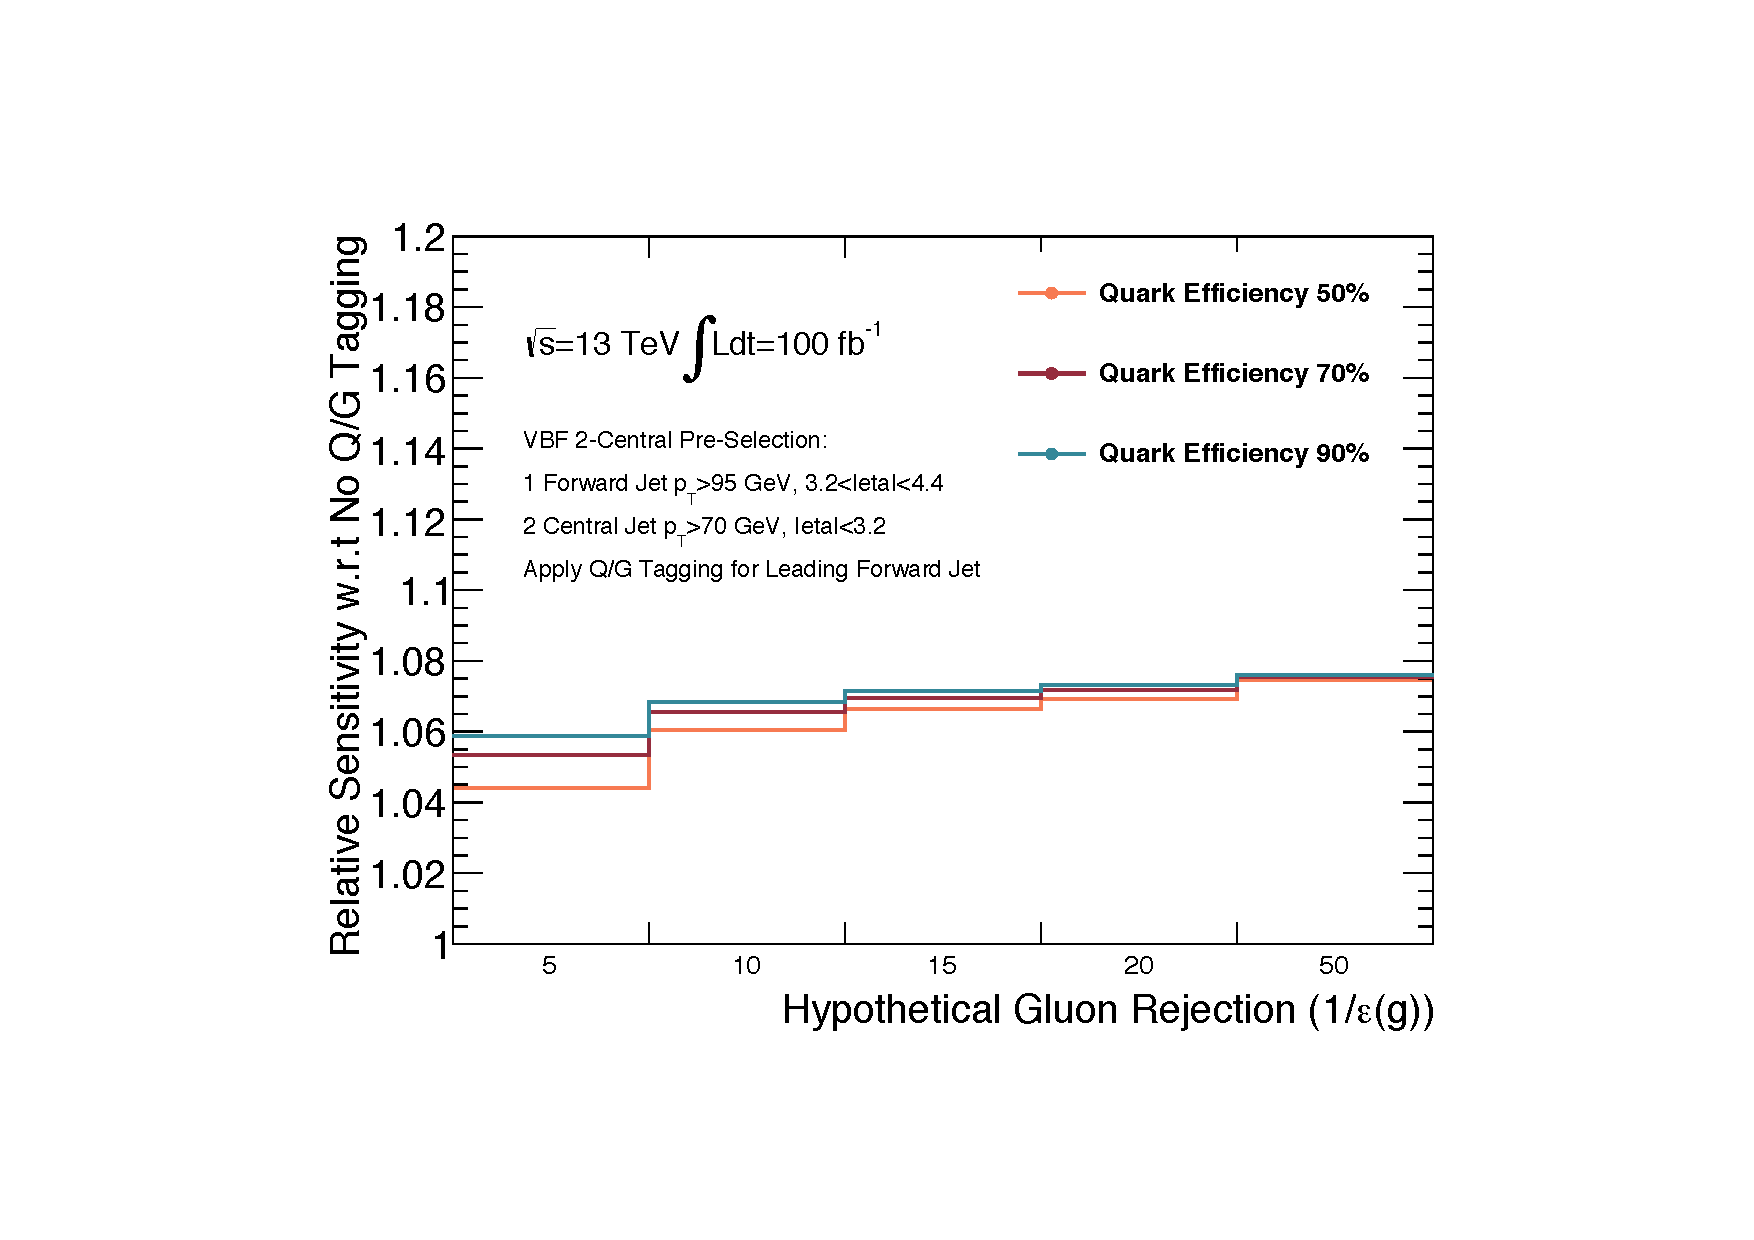
\includegraphics[width=0.8\textwidth]{figures/CNN/Relative_Gain.pdf}
\caption{Sensitivity gain study of applying quark/gluon tagging with different assumptions of quark efficiency and gluon rejections to the \twocentral channel of the VBF \Hbb search. The quark/gluon tagging is only applied to the forward jet of the event.}
\label{fig:cnn-gain}
\end{center}
\end{figure}
